% generated by Plantuml 1.2024.3       
\definecolor{plantucolor0000}{RGB}{241,241,241}
\definecolor{plantucolor0001}{RGB}{24,24,24}
\definecolor{plantucolor0002}{RGB}{173,209,178}
\definecolor{plantucolor0003}{RGB}{0,0,0}
\definecolor{plantucolor0004}{RGB}{200,41,48}
\definecolor{plantucolor0005}{RGB}{132,190,132}
\definecolor{plantucolor0006}{RGB}{3,128,72}
\begin{adjustbox}{width=.40\paperwidth, center}
	\resizebox{\textwidth}{!}{
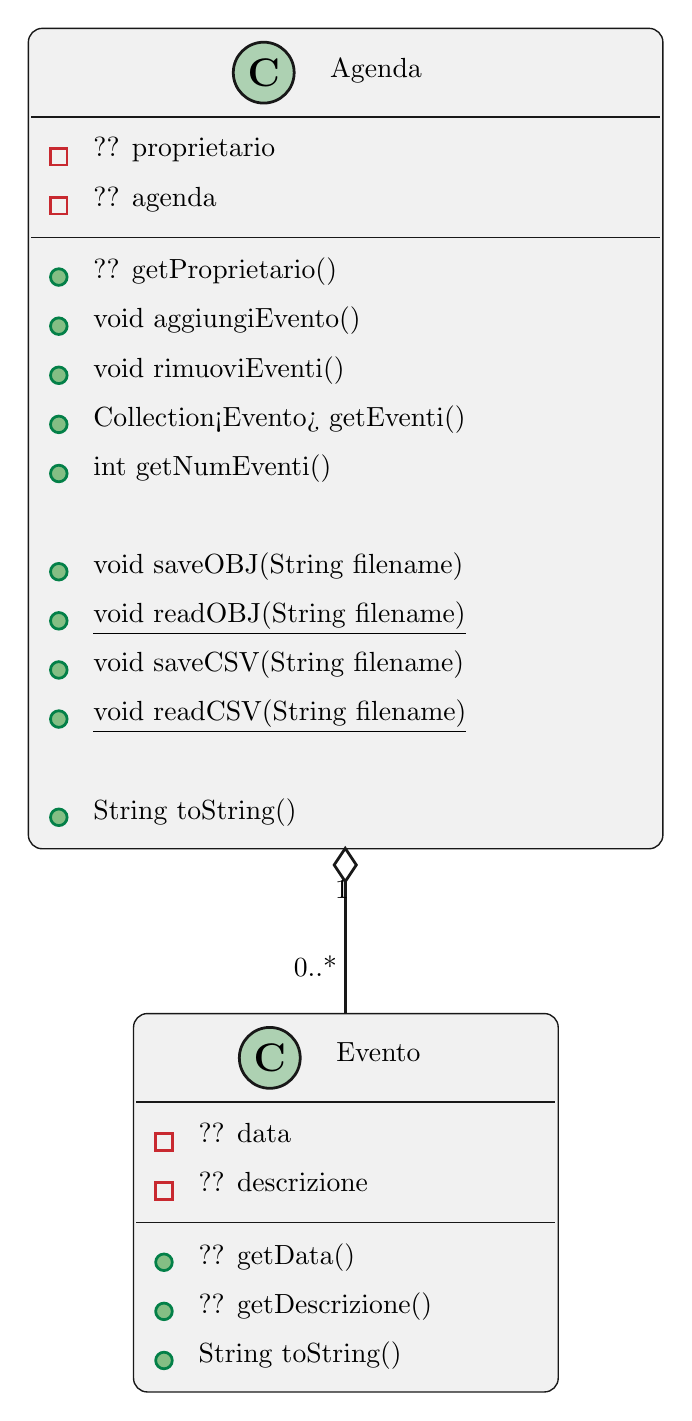
\begin{tikzpicture}[yscale=-1
,pstyle0/.style={color=plantucolor0001,fill=plantucolor0000,line width=0.5pt}
,pstyle1/.style={color=plantucolor0001,fill=plantucolor0002,line width=1.0pt}
,pstyle2/.style={color=plantucolor0001,line width=0.5pt}
,pstyle3/.style={color=plantucolor0004,line width=1.0pt}
,pstyle4/.style={color=plantucolor0006,fill=plantucolor0005,line width=1.0pt}
,pstyle5/.style={color=plantucolor0001,line width=1.0pt}
]
\draw[pstyle0] (45pt,368pt) arc (180:270:5pt) -- (50pt,363pt) -- (193.4606pt,363pt) arc (270:360:5pt) -- (198.4606pt,368pt) -- (198.4606pt,494.7305pt) arc (0:90:5pt) -- (193.4606pt,499.7305pt) -- (50pt,499.7305pt) arc (90:180:5pt) -- (45pt,494.7305pt) -- cycle;
\draw[pstyle1] (94.2341pt,379pt) ellipse (11pt and 11pt);
\node at (94.2341pt,379pt)[]{\textbf{\Large C}};
\node at (114.7341pt,370.127pt)[below right,color=black]{Evento};
\draw[pstyle2] (46pt,395pt) -- (197.4606pt,395pt);
\draw[pstyle3] (53pt,406.373pt) rectangle (59pt,412.373pt);
\node at (65pt,399pt)[below right,color=black]{?? data};
\draw[pstyle3] (53pt,424.1191pt) rectangle (59pt,430.1191pt);
\node at (65pt,416.7461pt)[below right,color=black]{?? descrizione};
\draw[pstyle2] (46pt,438.4922pt) -- (197.4606pt,438.4922pt);
\draw[pstyle4] (56pt,452.8652pt) ellipse (3pt and 3pt);
\node at (65pt,442.4922pt)[below right,color=black]{?? getData()};
\draw[pstyle4] (56pt,470.6113pt) ellipse (3pt and 3pt);
\node at (65pt,460.2383pt)[below right,color=black]{?? getDescrizione()};
\draw[pstyle4] (56pt,488.3574pt) ellipse (3pt and 3pt);
\node at (65pt,477.9844pt)[below right,color=black]{String toString()};
\draw[pstyle0] (7pt,12pt) arc (180:270:5pt) -- (12pt,7pt) -- (231.2828pt,7pt) arc (270:360:5pt) -- (236.2828pt,12pt) -- (236.2828pt,298.4453pt) arc (0:90:5pt) -- (231.2828pt,303.4453pt) -- (12pt,303.4453pt) arc (90:180:5pt) -- (7pt,298.4453pt) -- cycle;
\draw[pstyle1] (92.0485pt,23pt) ellipse (11pt and 11pt);
\node at (92.0485pt,23pt)[]{\textbf{\Large C}};
\node at (112.5485pt,14.127pt)[below right,color=black]{Agenda};
\draw[pstyle2] (8pt,39pt) -- (235.2828pt,39pt);
\draw[pstyle3] (15pt,50.373pt) rectangle (21pt,56.373pt);
\node at (27pt,43pt)[below right,color=black]{?? proprietario};
\draw[pstyle3] (15pt,68.1191pt) rectangle (21pt,74.1191pt);
\node at (27pt,60.7461pt)[below right,color=black]{?? agenda};
\draw[pstyle2] (8pt,82.4922pt) -- (235.2828pt,82.4922pt);
\draw[pstyle4] (18pt,96.8652pt) ellipse (3pt and 3pt);
\node at (27pt,86.4922pt)[below right,color=black]{?? getProprietario()};
\draw[pstyle4] (18pt,114.6113pt) ellipse (3pt and 3pt);
\node at (27pt,104.2383pt)[below right,color=black]{void aggiungiEvento()};
\draw[pstyle4] (18pt,132.3574pt) ellipse (3pt and 3pt);
\node at (27pt,121.9844pt)[below right,color=black]{void rimuoviEventi()};
\draw[pstyle4] (18pt,150.1035pt) ellipse (3pt and 3pt);
\node at (27pt,139.7305pt)[below right,color=black]{Collection<Evento> getEventi()};
\draw[pstyle4] (18pt,167.8496pt) ellipse (3pt and 3pt);
\node at (27pt,157.4766pt)[below right,color=black]{int getNumEventi()};
\node at (27pt,175.2227pt)[below right,color=black]{ };
\draw[pstyle4] (18pt,203.3418pt) ellipse (3pt and 3pt);
\node at (27pt,192.9688pt)[below right,color=black]{void saveOBJ(String filename)};
\draw[pstyle4] (18pt,221.0879pt) ellipse (3pt and 3pt);
\node at (27pt,210.7148pt)[below right,color=black]{\underline{void readOBJ(String filename)}};
\draw[pstyle4] (18pt,238.834pt) ellipse (3pt and 3pt);
\node at (27pt,228.4609pt)[below right,color=black]{void saveCSV(String filename)};
\draw[pstyle4] (18pt,256.5801pt) ellipse (3pt and 3pt);
\node at (27pt,246.207pt)[below right,color=black]{\underline{void readCSV(String filename)}};
\node at (27pt,263.9531pt)[below right,color=black]{ };
\draw[pstyle4] (18pt,292.0723pt) ellipse (3pt and 3pt);
\node at (27pt,281.6992pt)[below right,color=black]{String toString()};
\draw[pstyle5] (121.5pt,315.29pt) ..controls (121.5pt,336.15pt) and (121.5pt,344.7pt) .. (121.5pt,363pt);
\draw[pstyle5] (121.5pt,303.29pt) -- (117.5pt,309.29pt) -- (121.5pt,315.29pt) -- (125.5pt,309.29pt) -- (121.5pt,303.29pt) -- cycle;
\node at (114.3174pt,311.3496pt)[below right,color=black]{1};
\node at (99.3788pt,338.6737pt)[below right,color=black]{0..*};
\end{tikzpicture}
}
\end{adjustbox}